\chapter{Proposed - Patterns in potentiation across representations}
\label{chap:varying_representations}

\noindent
Authors: Austin Ferguson and Charles Ofria

\noindent
Status: This chapter is an alternative proposal for Chapter \ref{chap:simplified_model}. 
Both chapters look at potentiation in a representation other than Avida. 
While I lean toward Chapter \ref{chap:simplified_model} over this one, if I were to select this one I would swap the order around, doing this chapter after Chapter \ref{chap:varying_environments} so that I would have a baseline of how the multi-patch harvesting behavior becomes potentiated in Avida to compare with the other representation in this chapter. 
Additionally, all other chapters require minimal software development, while this chapter requires the implementation of Markov brains in MABE2. 

\section{Introduction}

Chapters \ref{chap:replaying_associative_learning} and \ref{chap:varying_environments} investigate the role of historical contingency in Avida. 
However, do the trends seen in Avida translate to other digital systems? 
This is the question we ask in this chapter.  

When writing all but the simplest software, we are plagued by making countless design decisions. 
Designing digital evolution systems is no different. 
How should organisms store data? 
Which instructions or operators do we include?
How large should the initial genome be, and what should it contain?
Is the genome directly encoded?
These are all valid questions when designing an evolving system, and each has multiple justifiable answers. 
However, with each a design decision comes a branching point in how that system operates. 
Depending on the specific decision, the difference between two choices can have a drastic effect on how evolution proceeds. 

Avida is no exception to this predicament; there are countless design decisions in Avida that affect the different dynamics of evolution. 
While some of these aspects have been empirically tested \citep{ofriaDesignEvolvableComputer2002, brysonUnderstandingEvolutionaryPotential2013}, others are nearly impossible to investigate because one small changes sends ripples throughout the other parameter spaces. 
%As an example, as seen when investigating evolved genomes in Chapter \ref{chap:alife_submission}, large portions of the genome can be un-expressed, resulting in a large fraction of mutations being neutral. 
%How does this interact with historical contingency? 
Here I propose we investigate the role in representation in potentiation by subjecting an alternate digital substrates to evolution and analysis on the same task. 
We leverage the patch harvesting task from Chapter \ref{chap:varying_environments}, whose inputs and outputs can easily be encoded to the various data types needed. 
I will evolve Markov brains \citep{hintzeMarkovBrainsTechnical2017} on the same environment, looking at the potentiation of mutli-patch harvesting behavior. 
%I will then analyze replicates from each substrate that successfully evolved memory usage. 
%Did successful lineages follow pathways similar to Avida? 
%How does potentiation change across substrates? 
By comparing these results to those in Chapter \ref{chap:varying_environments}, we can conduct a direct comparison in how potentiation changes as we change representations. 

My hypothesis is that the details of potentiation changes will vary as we change the underlying representation, but the general trends will stay the same. 
Markov brains are also capable of epistatic interactions, and I suspect that mutations that set up a potential interaction for the future will again cause large changes in potentiation. 
As mutations are quite different in the two systems, I expect to see difference in what these mutations are actually doing. 
For example, every mutation in Avida either changes, adds, or deletes a single instruction, while in Markov brains a mutation can change not only the type of a gate, but also how the other genes are interpreted.
Additionally, Markov brains have memory built in; some outputs are actually memory values that are then available as inputs in the next update. 
As such, I do \textit{not} expect Markov brains to potentiate with mutations that prep memory like we might see in Avida. 

% I expect substantial differences across substrates, however, I expect some general trends to hold true regardless the system used. 
% Specifically, I expect single mutations to greatly increase potentiation in each of the substrates. 
% Further, I expect to see the same general potentiation patterns (see discussion of Chapter \ref{chap:alife_submission}) across substrates. 
% By moving beyond Avida, we can begin to see general trends in potentiation and historical contingency in digital systems, and indeed, begin to set expectations for natural systems. 
\section{Methods}
Here I explain Markov brains, the alternate representation I will use in this work, as well as the changes to the patch harvesting environment required to accommodate the new substrate. 

\subsection{Markov brains}

% What are Markov brains?
At their most abstract level, the substrates we evolve on interactive tasks need three things: a way to receive inputs, a way to process data, and a way to output data. 
Avida organisms handle each of these with instructions, including specialized instructions for each environment to facilitate inputs and outputs. %some of which are specifically designed to pull information from the environment or take an action. 
Here we use Markov brains, which process data via binary logic gates connected to input and output buffers \citep{hintzeMarkovBrainsTechnical2017}. 


\begin{figure}[h!]
    \centering
    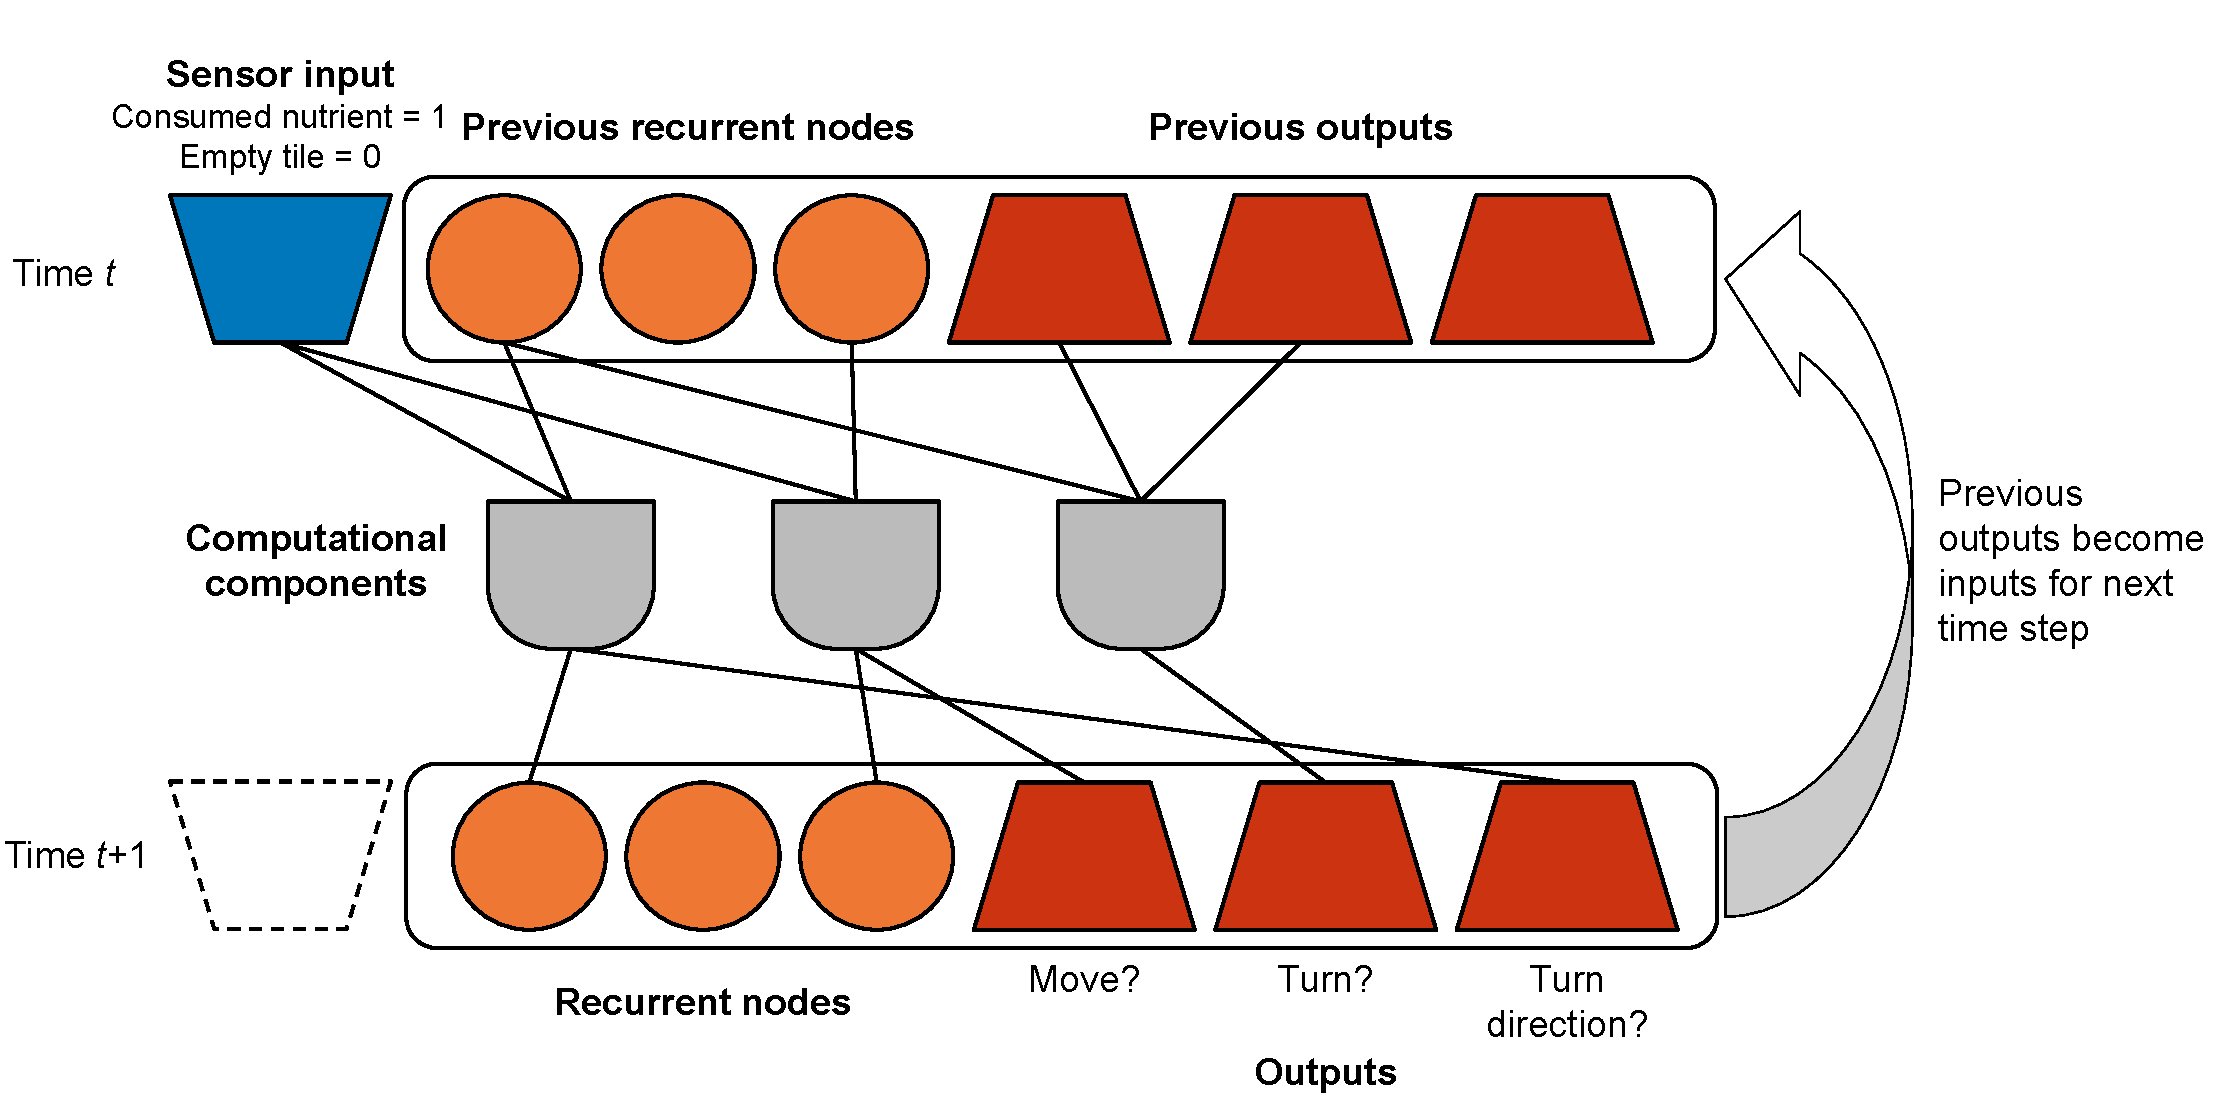
\includegraphics[width=0.95\textwidth]{07_potentiation_across_representations/media/markov_brain_conceptual_figure.pdf}
    \caption{Conceptual diagram of a Markov brain with inputs and outputs for the patch harvesting task, adapted from \citep{hintzeMarkovBrainsTechnical2017}.
    The single input, corresponding to the type of tile the organism is on, is shown as a blue trapezoid. 
    This example has three recurrent nodes (shown as orange circles) and three computational components (shown in gray). 
    The patch harvesting environment has three outputs, shown here as red trapezoids. 
    Note that the recurrent and output nodes (i.e., those in the rounded rectangle) will be passed as input in the next time step.
    The sensor input must come from the environment, as shown by the dashed trapezoid in the \textit{t+1} buffer.}
    \label{fig:varying_representations:markov_brain}
\end{figure}

% Go into more detail on how the brains work? Encoding?
Figure \ref{fig:varying_representations:markov_brain} shows an example Markov brain in the patch harvesting environment. 
At a given timestep \textit{t}, the organism will receive one input, some number of recurrent nodes, and three outputs (inputs and outputs described in the next subsection).
The genome of a particular brain encodes some number of computational components, including which inputs and outputs they are connected to. 
The inputs at timestep \textit{t} are passed into these computational components, and the outputs are written into an output buffer that includes recurrent nodes and output nodes (i.e., actuators). 
The environment will read the outputs and perform the appropriate actions, as described below. 
Finally, the recurrent and output nodes are passed back to the brain as part of the input buffer for time \textit{t+1}. 
This process constitutes one update, and each Markov brain will be executed for a given number of updates in order to perform its actions in the environment. 
A full description of Markov brains is available in \citep{hintzeMarkovBrainsTechnical2017}.

Computational components perform the transformation of inputs to outputs at each timestep. 
Here, I will only use deterministic logic gates for computational components, as they should be sufficient given that memory is already available via recurrent nodes. 
These logic gates take in some number of inputs and produce some number of outputs, with each deterministic logic gate containing its own truth table to map from inputs to outputs. 
For a given Markov brain, its computational components are all encoded in its genome. 
While we will avoid the details of the encoding (see \citep{hintzeMarkovBrainsTechnical2017} for details on computational components, logic gates, and the encoding scheme), it is important to note that Markov brains use a genetic encoding as compared to Avida's direct encoding. 
This allows for more flexibility in what effects mutations can have in a Markov brain. 
In our previous Avida work, a mutation always adds, removes, or swaps a single instruction. 
Mutations in Markov brains can have more minute difference, such as changing the type of computational component, modifying input/output connections, or changing the truth table of a logic gate. 
Combined with the fact that many sites in a Markov brain can be non-coding, these genomes have many possibilities for neutral and nearly-neutral mutations.
Additionally, the different effects that mutations can have create many a different suite of potential epistatic interactions than those found in Avida. 
Since we expect that epistatic interactions play a key role in the potentiation of a genome, these differences will likely influence how potentiation changes in Markov brains. 

\subsection{Changes to the patch harvesting environment and evolution system}

% We can't just throw Markov brains in the environment, we need to make a few changes
In Avida, the patch harvesting environment adds four new instructions: \texttt{Turn Left}, \texttt{Turn Right}, \texttt{Move Forward}, and \texttt{Sense}.
These instructions allow the organisms to pull information from the environment and take actions. 
Since Markov brains do not operate on the basis of instructions, we need to make some modifications to how the environment handles inputs and outputs. 

% How to modify IO
Instead of a \texttt{Sense} instruction that pulls the current tile's information into a register, to support Markov brains we will place the current tile's cue in the input buffer. 
Avida organisms work on 32-bit integers while Markov brains work on binary signals, so we will also need to convert the data itself. 
Because organisms consume food when they move on a tile, they can only encounter two types of tile cues: an empty tile or a tile that previous had food that has since been consumed. 
As such, we will place a one in the organism's input buffer if the tile previously contained food, or a zero if the tile has always been empty. 
Similarly, we need to determine what actions the organism will take based on the output buffer. 
To do this, we will give the organisms three bits of output. 
The first bit corresponds to movement; the organism will move forward if the movement bit is set. 
The last two bits will be used for turning. 
The first turning bit will determine if the organism will turn, while the second turning bit will determine which direction the organism will turn. 
Turning will be overridden by moving. 
Using two different bits to determine if the organism moves and if it turns allows for time steps with no environmental actions taken while still performing computation into the memory bits. 
With these modifications, the Markov brain organisms will have the pieces to sense their environment, do computation using normal Markov brain gates, and perform actions via their outputs. 

% Evolution system now needs to be synchronous 
The scoring of the environment and the classification of behaviors does not need to change from the Avida implementation. 
Organisms will still be rewarded for consuming food and punished for wandering into empty tiles. 
However, the evolution system itself will need to change to accommodate the change in representation. 
Avida operates on the concept of asynchronous generations -- organisms replicate themselves by executing certain instructions. 
This concept does not exist in Markov brains, so they must be externally replicated. 
As such, the Markov brains will evolve in a synchronous generation system. 
All organisms in the population will be evaluated independently to calculate their scores. 
Once the scores have been collected, we will select parents for the next generation by applying roulette (fitness proportional) selection, as it is the most similar to how Avida doles out updates. 
After replicating the parents and applying mutations, we will have our next generation and can restart the process.
We will conduct some preliminary experiments to ensure that Markov brains receive a comparable amount of time in the environment and comparable number of generations to the Avida organisms of Chapter \ref{chap:varying_environments}.


\section{Proposed work}

As in Chapter \ref{chap:varying_environments}, the main goal of this chapter is to replicate the potentiation analyses in Chapter \ref{chap:replaying_associative_learning} so we can then compare across systems. 
Here, this means we will be comparing potentiation along Markov brain lineages in the patch harvesting environment to Chapter 
\ref{chap:varying_environments} results on Avida lineages in the same environment.

Even though this chapter examines potentiation in Markov brains, a totally different substrate, our analyses of potentiation should be just as applicable. 
As such, I propose to conduct the same analyses as in Chapters \ref{chap:replaying_associative_learning} and \ref{chap:varying_environments}. 
Although this system uses synchronous generations, I can still track genotypic phylogenies and thus can conduct the two-phase replay experiments in the same way. 
As before, I will start by identifying the first genotype in the lineage that exhibits the target behavior and then seeding exploratory replay replicates 50, 100, 150, and 200 steps earlier in the lineage, launching additional replicates as needed until we reach the threshold of fewer than 10 percentage points of potentiation above the value found at the ancestor. 
I will then identify potentiation windows as done in previous chapters and run targeted replay replicates for each genotype in the windows. 

Once the replays have finished, the rest of the analysis is effectively identical to Chapter \ref{chap:varying_environments}. 
I will collect the measures of potentiation defined in Section \ref{sub:potentiation_measures}. 
Then I will statistically compare these measurements with the results of potentiation of Avida lineages on the patch harvesting tasks in Chapter \ref{chap:varying_environments}. 
Since each measurement is only comparing between two distributions (Avida versus Markov brains), we can simply conduct Mann-Whitney-Wilcoxon tests to look for statistical differences between the two \citep{10.2307/3001968}. 

This work will be the first direct comparison of how potentiation changes along successful lineages under different representations. 
I hypothesize that see similar trends in potentiation between the two representations. 
However, due to key differences, such as built-in memory in Markov brains or the differences in neutrality of the fitness landscape due to encodings, I expect the actual values of the measurements to differ between representations. 
% I do, however, expect the built-in memory to cause differences in some measurements, such as the number of potentiation windows. 
In Avida, evolving a strategy to successfully consume a single patch can be difficult to evolve (per preliminary work for Chapter \ref{chap:varying_environments}), and then evolving patch-switching behavior beyond that is an additional challenge. 
Thus I expect Avida to have two potentiation windows, on average, one for evolving the initial patch-harvesting behavior and a second for the patch-switching behavior.
My hypothesis is that the built-in memory of Markov brains eases the evolution of patch switching, resulting in one potentiation window in a typical Markov brain window, corresponding to the patch-harvesting behavior. 
In this case, I expect the Markov brain lineages to experience more potentiating gain in that single window, or more slow accumulation of potentiation. 
No matter what the results ultimately show, this work will be a solid step in exploring how potentiation changes; in combination with Chapters \ref{chap:replaying_associative_learning} and \ref{chap:varying_environments}, this work will complete the set of investigating potentiation when we vary the environment or the underlying organismal representation. 
These results will therefore be invaluable in future works in potentiation, whether they be theoretical, digital, or microbial.